\section{Design}\label{s:design}

\subsection{Modularized Design}
To support future adaptations and scalability, the code was structured into layers, each with  defined responsibilities and behavior.

\begin{figure}[h]
    \centering
    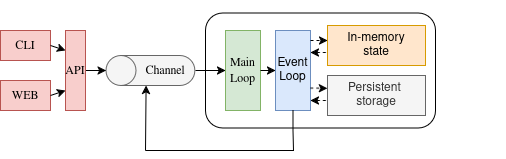
\includegraphics[width=0.5\textwidth]{../figures/Layers.png}
    \caption{Diagram showing layers of the simulator}
    \label{fig:layers}
\end{figure}

\textbf{1. CLI and Web}: These components serve as the primary user interfaces of the simulator. They run on separate threads and provide users with the ability to create nodes, establish links, start simulation runs, and perform many other management tasks.

The CLI operates in a loop that receives commands from the terminal and parses them accordingly. Rust enums provide type safety for commands, while the implementation of the `From` trait enables efficient conversion between user input and the corresponding command type.

The Web interface runs on an Axum server and serves static HTML content upon request. Once initialized, the JavaScript `Cytoscape` library enables the visualization and creation of nodes and links within the graph. HTTP is used for standard requests, while WebSockets provide fast communication during simulation runs.

\textbf{2. API}: This layers serves as a bridge between both the CLI/WEB and the channel. It exposes a unified set of functions that translate user requests into events executed int the simulation. 

Both interfaces comply with the same function signatures and data models, ensuring consistent behavior without direct coupling between them.

\textbf{3. Channel}: As the simulation engine and the entry points run on different threads, a communication channel must exist between them in order for user requests to be executed by the simulation.

This channel is a single-writer single-reader channel. Instead of sharing state between both layers, which would require locking due to Rust's mutable ownership rules, the entry point threads send event requests that are received by the main loop.

\textbf{4. Main Loop}: This loop is responsible for both receiving requests from the channel and executing the events processed by the event loop.

The loop first checks whether there are any pending events in the channel. If so, the channel is drained until no more events remain. It then checks whether there are any events in the EventLoop; if an event is present, it executes it.

After processing the event, the loop restarts. If no events are present either in the channel or in the event loop, it blocks the thread while waiting for new events to arrive on the channel. This is intended behavior, as new events can only be triggered by user requests and therefore appear in the channel.

\textbf{5. Event Loop}: This is the event loop responsible for ordering events based on the timestamp at which they must be executed.

It uses a binary heap. A binary heap is a data structure that provides $O(1)$ complexity for accessing the next event and $O(\log n)$ complexity for inserting events in the worst case.

\textbf{6. In-memory State}: This is the state used by the simulation for fast storage and retrieval of information during simulation runs.

It uses multiple HashMaps to store objects such as nodes, links, and measurements. A HashMap provides $O(1)$ complexity for data access and $O(1)$ complexity for data insertion.

As explained later, transitioning from fully persistent storage to an in-memory state resulted in a significant performance improvement.

\textbf{7. Persistent storage}: This is the storage used to persist data that must be shared across simulations. It stores information such as node and link data, generated keys, and other relevant simulation data.

\subsection{Design implementations}
This section explains how the different objects were simulated.

\textbf{Nodes and Detectors}: Nodes and detectors were implemented as independent objects; however, each node references a detector.

Each node has a \texttt{node type} attribute. The two possible types are \texttt{Client}, which is responsible for measuring qubits, and \texttt{EPR}, which is responsible for generating entangled pairs. A node is locked while it is participating in a simulation run, preventing other simulations from being executed concurrently on the same node.

Each detector has a cooldown rate. Upon reception of a qubit, if the detector is still on cooldown 
$$
(\texttt{last\_detection\_time + cooldown > timestamp})
$$

the qubit is dropped.

\textbf{Dark count rate}: The dark count rate is a constant property of the detector. As this rate increases, the average interval between dark count events decreases. Since these intervals should not be fixed but instead occur randomly in time, the process is modeled as a Poisson process. In a Poisson process, the time between consecutive events follows an exponential distribution. 

\begin{figure}[ht]
    \centering
    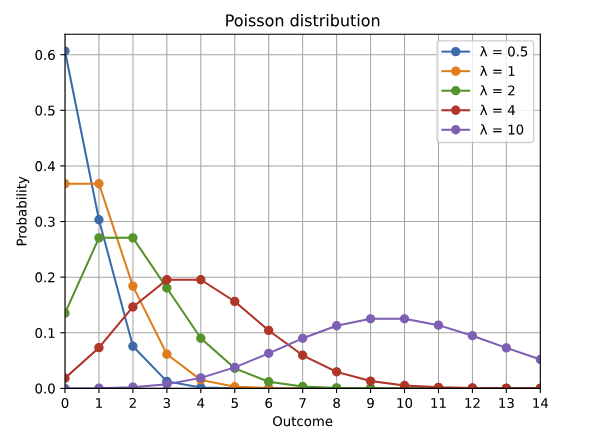
\includegraphics[width=0.5\textwidth]{../figures/poisson.png}
    \caption{Diagram showing the poisson distribution}
    \label{fig:poisson}
\end{figure}


As shown in Figure~\ref{fig:poisson}, when the parameter $\lambda$ becomes smaller (which corresponds to a higher dark count rate), the distribution becomes more concentrated near zero, resulting in shorter intervals between dark count events.

\textbf{Links}: Links model the connection between two nodes. Each link has a \texttt{distance} attribute, which affects both the data propagation delay and the fidelity degradation over the channel.

As explained in Subsection~\ref{s:obstacles}, a constant fidelity degradation factor of 0.14\% per kilometer was used. Therefore, the longer the link, the lower the entanglement fidelity of transmitted qubits.

\textbf{Entanglement \& Measurement}: An entangled pair in a Bell state is modeled as a struct instance. This instance stores the measurements from both nodes, and the measurement logic is defined as follows:

\begin{enumerate}
    \item Check whether the current measurement is the first.

    \textbf{If it is the first measurement:}
    \begin{enumerate}
        \item Choose a random basis.
        \item Generate a random number between 0 and 1.
        \item Store the measurement in the corresponding measurement attribute of the pair.
    \end{enumerate}

    \textbf{If it is the second measurement:}
    \begin{enumerate}
        \item Calculate the updated fidelity after distance-based degradation.
        \item Choose a random basis.
        \item Compute the basis difference between the first measurement basis and the current one.
        \item Compute the entanglement probability.
        \item Based on this probability, either copy the first measurement outcome or take the opposite result.
        \item Store the measurement in the corresponding measurement attribute of the pair.
    \end{enumerate}
\end{enumerate}

The entanglement probability function is as follows:

\[
P_{\text{same}} = F \cdot \cos^{2}(\alpha - \beta) + (1 - F) \cdot 0.5
\]

Where:
\begin{itemize}
    \item \textbf{$\alpha$ and $\beta$} are the chosen angles.
    \item \textbf{$F$} is the fidelity after degradation.
    \item \textbf{$\cos(\cdot)$} represents the correlation function.
\end{itemize}

This function behaves correctly because when the fidelity is zero, the probability becomes $0.5$, meaning the output is completely random.

\textbf{Mallory}: The most appropriate way to model the presence of Mallory in a connection was to define links as either secure or insecure, and to execute different logic depending on the type of link.

When a link is defined as insecure, a measurement is performed and stored in the pair before the actual measurement. Then, in subsequent measurements, the basis calculation and entanglement probability are computed using Mallory's measurements instead of the actual client node measurements.

This result in a completely random outcome.

\subsection{Obstacles}\label{s:obstacles}
This section exposes some of the many obstacles found during the design and development process.

The first obstacle arose during the design phase. During the investigation, it was found that many simulators model fidelity degradation through multiple physical effects, such as fiber optic attenuation, quantum memory efficiency, and other channel imperfections. However, since this project focuses on the E91 protocol simulation and CHSH inequality validation, a highly detailed physical model of fidelity degradation was not required.

After extensive research, the paper \cite{sena2025entanglement} showed that after 100 km of fiber optic transmission, the entanglement fidelity decreases to approximately 86\%, corresponding to a reduction of about 0.14\% per kilometer. Therefore, a constant fidelity degradation rate of 0.14\% per kilometer was chosen for the simulation.

During the development of the simulator, several obstacles were encountered, mainly due to Rust's programming rules.

In a simulation where events are scheduled based on runtime conditions, the system needs a way to execute functions dynamically. In Python, this can be achieved using reflection, where a dotted string path is resolved at runtime into a callable object .However, Rust is a statically compiled language and does not provide built-in runtime reflection of function names. 

The solution was to create a registry that stored a function HashMap. This HashMap would map a EventName instance to its corresponding function stored in a Box pointer.

The last obstacle was performance. At the beginning, persistent storage was used as the storage for everything. This meant that not only nodes and links were stored, but also measurements and entangled pairs. As a result, a simulation with 10,000 qubits took more than 5 minutes to complete due to database acceses and locks between threds.

The solution was to move away from a shared database state between threads and instead adopt an in-memory HashMap-based state managed directly by the simulation loop.
